% This is a general templete to start a new Kurt Pan's paper.


\documentclass[runningheads]{llncs}
\pagestyle{plain}
\usepackage[dvipsnames]{xcolor}
\usepackage[lambda,sets,operators]{cryptocode}
\usepackage{amsmath}
\usepackage{amssymb}
\usepackage{graphicx}
\usepackage[hyperref=true,backend=biber,backref=true,style=alphabetic,minalphanames=3,maxalphanames=4]{biblatex}
\DefineBibliographyStrings{english}{
  backrefpage={Cited on page},
  backrefpages={Cited on pages}
}

\addbibresource{kurt.bib}

\usepackage{hyperref}
\hypersetup{colorlinks=true,citecolor=magenta,linkcolor=magenta,urlcolor=magenta,pdftitle={Title},pdfauthor={Kurt Pan},linktoc=all}

\usepackage{fontspec}
\usepackage{xeCJK}
\setCJKmainfont{LXGW WenKai Mono}
\linespread{1.5}
\usepackage{enumitem}





\begin{document}

\title{简明zkSNARKs分类手册(v1.1)}
\author{Kurt Pan}
\institute{Cryptoland}
\maketitle

\begin{abstract}
通过本次作业对zk-SNARKs相关定义概念和相关工作进行简洁的整理和区分,希望在完善后能作为一个参考手册帮助zk研究者和从业者。

\begin{itemize}
  \item 2023.06.20 v1.1
  \item 2022.07.21 v1.0
\end{itemize}



\keywords{zk-SNARKs }
\end{abstract}

\setcounter{tocdepth}{2}
\tableofcontents


% core content starts here

\section{总论}



\subsubsection*{已知有五条路径可以构造一个论证系统},都是由一个信息论安全的协议和密码学方案一起组合而成:
\begin{enumerate}
  \item 基于交互式证明系统IP的(GKR协议)
  \item 基于多证明者交互式证明系统MIP的
  \item 基于常数轮多项式交互式谕示证明PIOP的 (包括MPC-in-the-Head)
  \item 基于线性概率可检验证明系统LPCP的。
  \item 基于承诺并证明技术的
\end{enumerate}


\subsubsection*{已知有三条路径来构造一个多项式承诺方案:}
\begin{enumerate}
  \item 基于IOP和Merkle哈希组合:FRI \cite{BBH17} /Ligero \cite{AHI17} /Brakedown \cite{GLS21}
  \item 基于透明$\Sigma$协议,离散对数假设:Hyrax \cite{WTS18}, Bulletproof \cite{BBB18}, Dory
  \item 基于配对和可信设置:KZG \cite{KZG10}
  
\end{enumerate}
\subsubsection*{绝大多数SNARK设计三步走方法:}
\begin{enumerate}
  \item 设计一个对电路可满足性或R1CS可满足性问题的公开抛币PIOP
  \item 用多项式承诺方案替换PIOP中的每一条消息$h_i$,得到一个公开抛币的交互式简洁论证系统
  \item 用Fiat-Shamir去掉交互性
\end{enumerate}

\section{关键组件的定义}
\subsection*{信息论证明系统}
\begin{itemize}
  \item \textbf{IP} : 交互式证明系统
  \item \textbf{MIP} \cite{BGK88} : 多证明者交互式证明系统,多个证明者分别和一个验证者进行交互式证明。
  \item \textbf{PCP} \cite{AS98}: 概率可验证证明系统,验证者查询访问证明者的消息字符串。
  \item \textbf{IOP} \cite{BCS16}: 交互式谕示证明系统, 结合了IP和PCP的特点,验证者和证明者同时具有交互和查询访问消息。
\end{itemize}

\subsubsection*{理论模型}
\begin{itemize}
  \item \textbf{CRS}:所有参与方可以访问一个公共的参考串
  \item \textbf{ROM}:随机预言模型 
  \item \textbf{AGM}:代数群模型
  \item \textbf{Fiat-Shamir范式}: 将任何公开抛币交互式论证系统转换为一个对同样语言的非交互论证系统。该转换在对常数轮协议,在随机预言模型中,是可靠的。\cite{BR93}

\end{itemize}

\subsection*{zk-SNARKs}
\begin{itemize}
  \item \textbf{零知识}:验证者除了陈述正确性不能获得任何其他知识增长
  \item \textbf{简洁}:验证者运行时间比进行计算更短
  \item \textbf{非交互}:协议通信只有证明者向验证者发送的一条消息
  \item \textbf{论证系统}:证明系统其中可靠性只对恶意的多项式时间证明者成立(依赖密码学假设)
  \item \textbf{知识证明}:证明者确实拥有知识
\end{itemize}
\subsection*{多项式承诺方案}
多项式承诺方案是输入对象为多项式的密码学承诺方案,满足隐藏性和绑定性。此外还满足部分打开部分点处的求值,不用全部打开整个多项式。常见多项式承诺方案有如下分类:

\begin{itemize}
  \item KZG \cite{KZG10} 基于配对椭圆曲线,结构化公共字符串
  \item IPA \cite{BBB18} 内积论证系统
  \item FRI \cite{BBH17} 快速里德所罗门交互式谕示证明系统
\end{itemize}

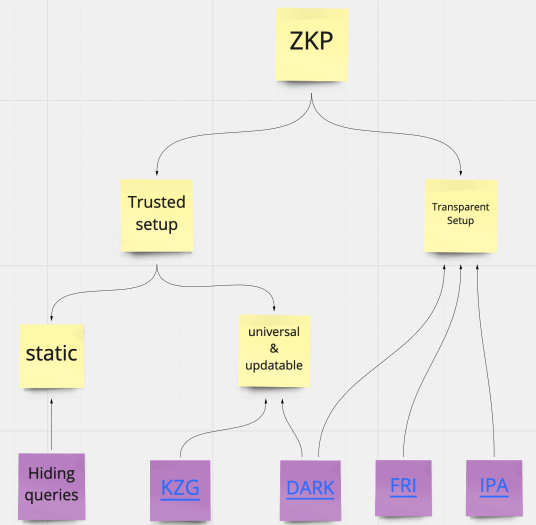
\includegraphics[scale=0.5]{pc.png}


\subsection*{可信设置}

\begin{itemize}
  \item \textbf{计算特定}可信设置:SRS中包含power-of-tau,以及表示电路连线模式或R1CS矩阵项的多项式求值的编码。
  
  \item \textbf{通用}(universal)可信设置:一个SRS可以对任意R1CS/电路可满足性实例使用,直到某个固定的大小界。只包含power-of-tau,电路无关。
  
  \item \textbf{可更新}(updatable)可信设置:SRS可以在任意时间由任何参与方更新,只要至少有一个参与方诚实,证明就不可以被伪造。
\end{itemize}

\subsection*{算术化和中间表示}
\begin{itemize}
  \item \textbf{算术化}:将通用陈述或问题转换为可验证的方程组的过程。
  \item \textbf{算术电路}:线路为有限域中的元素,门为加法门和乘法门的电路
  \item \textbf{R1CS/QAP}:一种用一系列算术方程编码算术电路的方法
\end{itemize}


\section{组合为不同方案: SNARKS 菜谱}


\begin{itemize}
  \item Virgo \cite{ZXZ20} = IP + FRI
  \item Hyrax \cite{WTS18} = IP + IPA
  \item Libra \cite{XZZ19} = IP + KZG
  \item Spartan \cite{Setty20}, Quarks \cite{SL20} = MIP + IPA
  \item Brakedown, Shockwave \cite{GLS21} = MIP + Brakedown/Ligero-承诺
  \item Aurora \cite{BCR19}, Fractal \cite{COS20}, Redshift \cite{KPV19}, STARK\cite{BBH19}, Plonky2 \footnote{\url{https://github.com/mir-protocol/plonky2/blob/main/plonky2/plonky2.pdf}} = PIOP + FRI
  \item Ligero \cite{AHI17} = PIOP + Ligero-承诺
  \item Ligero++ \cite{BFH20}= PIOP + Ligero-承诺 + FRI
  \item Sonic \cite{MBK19} ,  Marlin \cite{CHM20} ,  PlonK \cite{GWC19} = PIOP + KZG
  \item Halo 2 \footnote{\url{https://zcash.github.io/halo2/}} = Plonk PIOP + IPA
  \item Pinocchio \cite{PHG13}, Groth16 \cite{Groth16} = LPCP + 配对
\end{itemize}

% 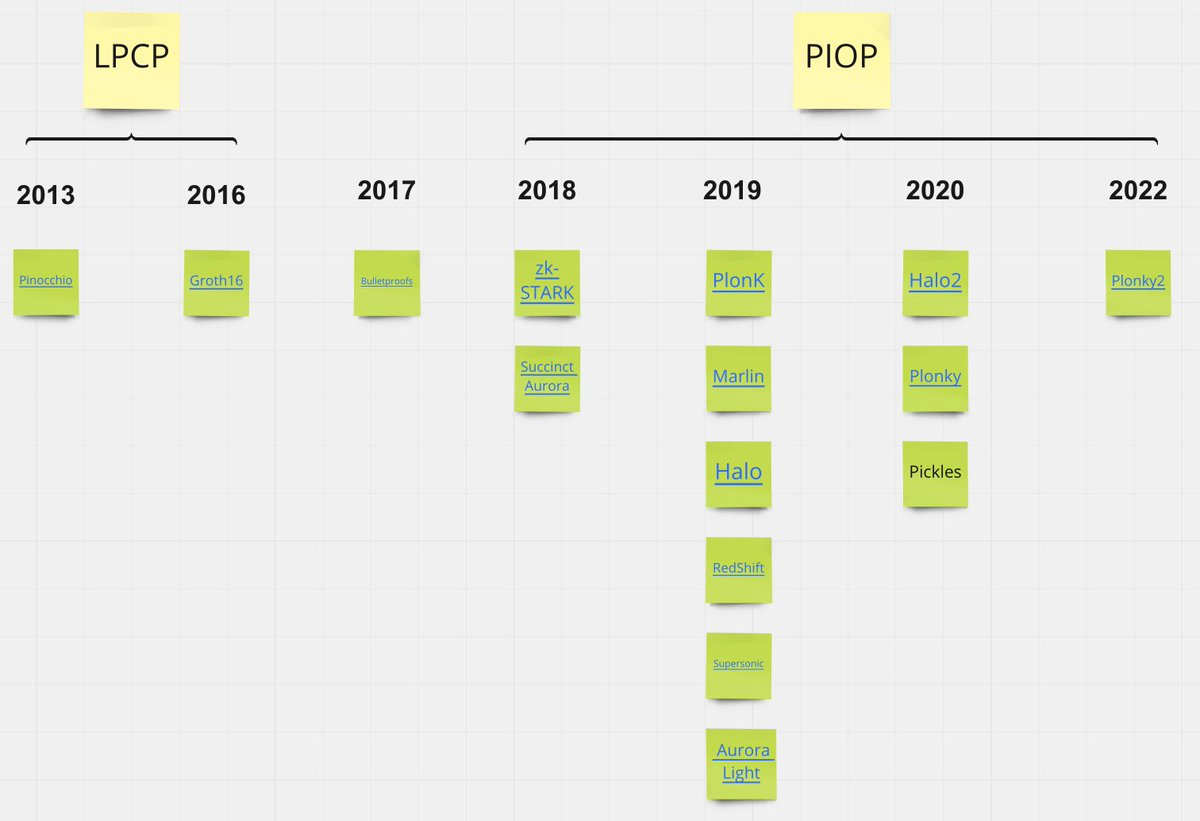
\includegraphics[scale=0.37]{LPCPPIOP.jpg}
% 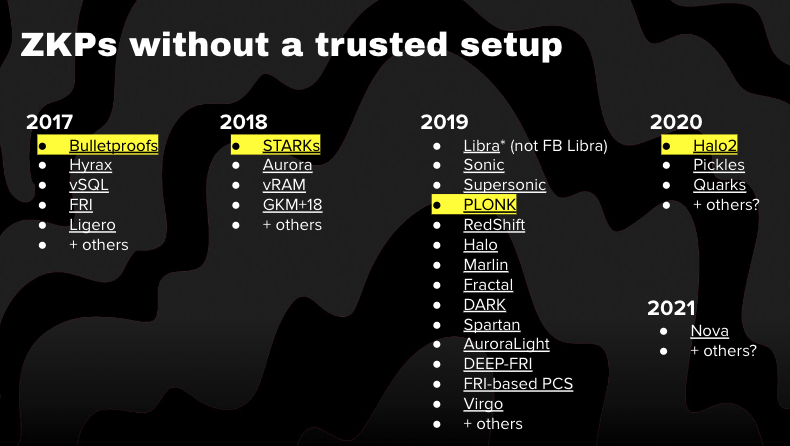
\includegraphics[scale=0.5]{wotrustedsetup.png}







\section{各个因素的权衡}

\subsection{常数证明大小}
有两条路径可以达到「证明大小只包含常数个群元素」:常数轮PIOP+KZG多项式承诺,LPCP+双线性配对。前者的代表Marlin证明大小大约是后者代表Groth16(只要3个群元素)的4倍,Plonk 的证明大小大约是Groth16的2.5倍。所以在「最小证明大小」这个目标上后者完胜。

这两条路径都有如下两个缺点
都用了SRS,都需要可信设置。但前者使用SRS的缺点没有后者严重:前者的SRS是通用的且可更新的,后者的SRS是计算特定的。
证明者计算开销都很大。证明者要进行多个FFT/多项式除法/多指数运算,时间和空间开销都很大且不易并行化和分布化。
\subsection{透明性Transparency}
除了上述两条为了极小化证明大小的路径,只要不使用基于KZG的多项式承诺,其他的路径构造出的SNARK都是透明的。使用URS而非SRS。
\subsection{后量子安全}
IOP是可能后量子的,所以基于IOP的多项式承诺方案(FRI/Ligero/Brakedown)(包括MPC-in-the-Head方法构造的IOP)都是后量子的,另外两类多项式承诺方案因为依赖离散对数问题的困难性非后量子的。

\subsection{域选择的限制}
比如关于加密和签名方案的证明,很多加密和签名方案是定义在非FFT友好的有限域上的椭圆曲线群中的,如果SNARKs系统证明者需要进行FFT,则就不能用。

\subsubsection*{来自可靠性保证}
域大小必须足够大以确保达到想要的可靠性安全级别。

\subsubsection*{来自零散对数或KZG多项式承诺} 使用基于零散对数或KZG多项式承诺的SNARKs,以及LPCP+配对的方法,都必须使用和多项式承诺定义的群阶数相等的域。

\subsubsection*{来自FFT} 来自IOP和线性PCP的SNARKs要求证明者在大向量上进行FFT运算,而不同的有限域对FFT算法的支持具有不同的复杂度。部分常数轮PIOP \cite{CHM20,GWC19}要求有限域具有特定乘法或加法子群。
\subsubsection*{来自程序-电路转译} 在一些基于IOP的SNARKS中(比如STARKs \cite{BBH19}),从计算机程序(RAMs)到电路或其他中间表示的转换过程只适用于特征为2的域。

\subsection{不同操作的相对效率} 
证明者的瓶颈可能是在域上FFT,可能是群操作(多指数),也可能是构造Merkle树中的哈希求值。哪个操作成为瓶颈也依赖于要处理的计算的大小。

\subsection{中间表示(IR)}
除了上述的算术电路和R1CS,还可以支持更通用的中间表示。比如扩展门,支持大于2的门的扇入,从而产生更快的证明者。比如“类Plonk算术化” 指对Plonk \cite{GWC19}的修改以支持一种电路门的度数可以达到9的中间表示。


\printbibliography
\end{document}
